\documentclass[journal]{IEEEtran}
\usepackage[utf8]{inputenc}
\usepackage[T1]{fontenc}
\usepackage{amsmath,amssymb,amsthm,bm}
\usepackage{cite}
\usepackage{graphicx}
\usepackage{algorithm}
\usepackage{algorithmic}
\usepackage{booktabs}
\usepackage{multirow}
\usepackage{xcolor}
\usepackage{url}
\usepackage{tikz}
\usetikzlibrary{arrows.meta,positioning,calc,shapes.geometric}
\usepackage{caption}
\usepackage{subcaption}
\usepackage{enumitem}
\graphicspath{{figures/}}

\newtheorem{theorem}{Theorem}
\newtheorem{lemma}{Lemma}
\newtheorem{proposition}{Proposition}
\newtheorem{corollary}{Corollary}
\newtheorem{remark}{Remark}
\newtheorem{definition}{Definition}
\newtheorem{assumption}{Assumption}

% ---- placeholders for the mathematical parts assigned to the co-author ----
\newcommand{\todo}[1]{\textcolor{red!70!black}{[To do: #1]}}
\newcommand{\todobox}[1]{\begin{center}\fbox{\parbox{0.95\columnwidth}{\small\textcolor{red!70!black}{\textbf{[To do]} #1}}}\end{center}}

% ---- notation ----
\newcommand{\E}{\mathbb{E}}
\renewcommand{\Pr}{\mathrm{Pr}}
\newcommand{\R}{\mathbb{R}}
\newcommand{\C}{\mathbb{C}}
\newcommand{\creq}{c_{\mathrm{req}}}
\newcommand{\creqk}[1]{c_{\mathrm{req},#1}}
\newcommand{\Dmax}{D_{\max}}
\newcommand{\Pmax}{P_{\max}}
\newcommand{\vect}[1]{\bm{#1}}
\newcommand{\Sset}{\mathcal{S}}
\newcommand{\Kset}{\mathcal{K}}
\newcommand{\Mset}{\mathcal{M}}
\newcommand{\neff}{n_{\mathrm{eff}}}
\newcommand{\dB}{\,\mathrm{dB}}
\newcommand{\dBm}{\,\mathrm{dBm}}

\begin{document}

\title{Tail-Latency-Aware Segmented Waveguide-Enabled Pinching-Antenna Systems for Hyper-Reliable Low-Latency Communications Under Bursty Traffic}

\author{First~Author,~\IEEEmembership{Member,~IEEE,}
        Second~Author,~\IEEEmembership{Member,~IEEE}%
\thanks{Manuscript received September~2026. (\emph{Corresponding author: First Author.})}%
\thanks{F. Author and S. Author are with the Department of Electronics and Telecommunications, University Name, City, Country (e-mail: \{first, second\}@university.edu).}}

\markboth{IEEE Transactions on Wireless Communications}%
{Author \MakeLowercase{\textit{et al.}}: Tail-Latency-Aware SWAN for HRLLC Under Bursty Traffic}

\maketitle

\begin{abstract}
Segmented waveguide-enabled pinching-antenna systems (SWANs) replace the single long dielectric waveguide of a pinching-antenna system (PASS) by several short, individually fed segments, each of which activates one pinching antenna (PA). SWANs thereby provide reconfigurable line-of-sight channels without inter-antenna radiation and can serve users either by aggregating all segments or by multiplexing them. Existing SWAN and PASS designs, however, optimize average rates under full-buffer traffic, whereas 6G hyper-reliable low-latency communication (HRLLC) is specified by the \emph{tail} of the packet delay under bursty, deadline-constrained arrivals. This paper studies a downlink multi-user SWAN whose users generate packets according to Markov-modulated ON--OFF processes, transmit with finite-blocklength (FBL) codes, and discard packets whose delay budget expires. We formulate the joint PA placement, segment-mode selection, user scheduling, and rate/power adaptation problem under per-user delay-violation-probability constraints and propose a two-timescale tail-latency-aware scheme, TLA-SWAN. On the frame timescale, a closed-form mapping from each user's burst statistics and tail target to a \emph{tail-latency-aware required service rate} drives a low-complexity block-coordinate PA placement that maximizes the minimum tail-latency margin. On the slot timescale, a packet-value scheduler derived from Lyapunov drift-plus-penalty arguments assigns exponentially deadline-weighted values to queued packets, augments them with a virtual credit that tracks each user's service deficit with respect to its required rate, and jointly selects the served user set (aggregation or multiplexing), the number of packets per codeword, and the power level through an exhaustive search over pre-computed zero-forcing tables. Extensive slot-level simulations with FBL decoding errors and deadline-constrained queues show that TLA-SWAN reduces the delay-violation probability by more than an order of magnitude with respect to rate-centric SWAN designs, classical deadline-aware schedulers, single-waveguide PASS, and fixed antenna arrays, that its statistical placement is robust to reconfiguration delays that cripple reactive repositioning, and that it exposes a tunable power--tail trade-off.
\end{abstract}

\begin{IEEEkeywords}
Pinching-antenna systems, segmented waveguide, hyper-reliable low-latency communication, tail latency, bursty traffic, finite blocklength, Lyapunov optimization, scheduling.
\end{IEEEkeywords}

\IEEEpeerreviewmaketitle

%=====================================================================
\section{Introduction}
%=====================================================================
\IEEEPARstart{H}{yper-reliable} and low-latency communication (HRLLC) is one of the six usage scenarios of IMT-2030, with research targets of $0.1$--$1$~ms air-interface latency and reliability between $1-10^{-5}$ and $1-10^{-7}$ \cite{ITUR-M2160}. Such targets are not statements about the \emph{average} delay: they bound the probability that the delay of a packet exceeds a budget, i.e., the tail of the delay distribution \cite{Bennis2018}. Two features of HRLLC applications make the tail particularly hard to control. First, the traffic is bursty: industrial closed-loop control, event-triggered alarms, and extended-reality (XR) frames produce packets in clusters separated by silent periods \cite{3GPP-TS22104,3GPP-TR38838,Zhang2025HRL}, so that even a lightly loaded link experiences short overload periods during which queues build up. Second, HRLLC packets are short, so that finite-blocklength (FBL) coding penalties and decoding errors must be accounted for jointly with queueing \cite{Polyanskiy2010,Durisi2016,Zhao2022QueueAware,Li2024RLR}. The wireless link therefore needs enough \emph{instantaneous} capacity to drain a burst within the delay budget, which in turn calls for physical-layer architectures that can bring high signal-to-noise ratio (SNR) to wherever a burst occurs.

Pinching-antenna systems (PASS) are a recently proposed flexible-antenna technology in which small dielectric particles (pinching antennas, PAs) are attached at adjustable positions along a dielectric waveguide fed by the base station (BS) \cite{Ding2025FlexibleAntenna,Liu2026PASSTutorial,Liu2026PASSSurvey,Xu2025GeneralizedPASS}. By activating a PA close to a user, PASS shortens the free-space path and establishes a strong line-of-sight (LoS) link, which makes it attractive for millimeter-wave deployments in factories and indoor venues. A single long waveguide, however, suffers from in-waveguide propagation loss and from inter-antenna radiation (IAR) when several PAs are activated. Segmented waveguide-enabled PASS (SWAN) \cite{Ouyang2026SWAN} solves both problems by dividing the waveguide into short segments, each with its own feed connected to the BS by fiber or cable, and by activating a single PA per segment. The feeds can be driven by separate radio-frequency (RF) chains, so that a SWAN behaves like a distributed antenna array whose element positions are reconfigurable within their segments. This gives rise to three operating modes \cite{Ouyang2026SWAN,Shan2026SWANAccess}: segment selection (one segment serves a user), segment aggregation (SA, all segments coherently serve one user), and segment multiplexing (SM, the segments spatially multiplex several users). Existing SWAN studies characterize the SNR and sum-rate of these modes \cite{Ouyang2026SWAN,Gu2026SWANSumRate,Gu2026HSSA}, design hybrid beamformers \cite{Jiang2026SWANTriHybrid,Guo2026SWANGNN}, integrate sensing \cite{Jiang2025SWANISAC,Gao2026SWANISAC,Geng2026CRLBSWAN}, and design random-access protocols \cite{Shan2026SWANAccess}. All of them assume saturated (full-buffer) traffic and infinite-blocklength coding; none considers queueing, deadlines, or the delay tail.

The combination of SWAN and HRLLC raises three questions that the rate-centric literature does not answer. (i) \emph{Where should the PAs be placed} when users differ in burstiness and in tail targets? A placement that maximizes the sum-rate moves PAs towards users with good channels, whereas the delay tail is governed by the users whose bursts are hardest to drain. (ii) \emph{How should the BS decide, slot by slot, between aggregation and multiplexing}, how many short packets to bundle in a codeword, and at which power, when a decoding failure delays all bundled packets and the reliability target is $10^{-5}$? (iii) \emph{How fast can the SWAN be reconfigured?} Physical PA repositioning takes from microseconds (pre-installed PAs that are switched on and off) to seconds (sliding PAs) \cite{Liu2026PASSTutorial,Wang2026Roaming,Wang2026FiniteSpeedPA,Jiang2026DiscreteCoupling}, so that chasing bursts by moving PAs may cost more than it gains.

\subsection{Related Work}
\subsubsection{PASS and SWAN}
The channel and signal models of PASS were established in \cite{Ding2025FlexibleAntenna} and are surveyed in \cite{Liu2026PASSTutorial,Liu2026PASSSurvey,Xu2025GeneralizedPASS}. SWANs were introduced in \cite{Ouyang2026SWAN}, which derived the SNR scaling laws of the segment-selection, aggregation, and multiplexing modes and showed that segmentation shortens both the PA-to-user and the PA-to-feed distances. Follow-up work addressed uplink sum-rate maximization with TDMA and NOMA \cite{Gu2026SWANSumRate}, joint segment activation and PA placement under a single RF chain \cite{Gu2026HSSA}, tri-hybrid (digital, analog, pinching) beamforming \cite{Jiang2026SWANTriHybrid}, learning-based placement \cite{Guo2026SWANGNN}, integrated sensing and communication \cite{Jiang2025SWANISAC,Gao2026SWANISAC,Geng2026CRLBSWAN}, maintainability \cite{Ouyang2026Maintainability}, frequency selectivity over long apertures \cite{Ouyang2026FSPASS}, and access protocols that exploit the reconfigurable channel diversity of SWANs \cite{Shan2026SWANAccess}. Timeliness has been considered only through the age of information for vehicular platooning over SWANs \cite{Zheng2026SWANPlatoon}. For single-waveguide PASS, FBL rate optimization for a single user was studied in \cite{Lin2025URLLCPASS} and a statistical-CSI short-packet design in \cite{Pan2026ShortPacketPASS}; both consider one user, one packet, and no queue. The cost of PA repositioning has been modeled through a finite movement speed \cite{Wang2026Roaming,Wang2026FiniteSpeedPA} and discrete activation \cite{Jiang2026DiscreteCoupling}, again without arrivals or deadlines. A recent network-level perspective \cite{Xu2026NetworkPerspective} lists queue-aware PA scheduling under discrete activation constraints as an open problem, which is precisely the problem addressed here.

\subsubsection{Tail latency under bursty traffic and finite blocklength}
The delay tail of a wireless queue is classically characterized by effective bandwidth and effective capacity \cite{Chang1994,Kelly1996,Wu2003,Ozmen2016}, by stochastic network calculus \cite{Fidler2015,AlZubaidy2016,Schiessl2018}, and by extreme value theory \cite{Bennis2018,Liu2019MEC}. Markov-modulated ON--OFF sources are the standard model of bursty arrivals, with closed-form effective bandwidths due to Anick, Mitra, and Sondhi \cite{Anick1982,Elwalid1993}. In the URLLC context, \cite{She2018CrossLayer} converted a queueing-delay-violation constraint into a service-rate requirement through the effective bandwidth of the arrivals and combined it with the FBL decoding error; \cite{Gursoy2013,Schiessl2018} incorporated FBL coding into effective capacity and network calculus; \cite{Zhao2022QueueAware} adapted the blocklength to the queue state; and \cite{Li2024RLR,Li2024Tractable} characterized the reliability--latency--rate trade-off and tractable queue-tail approximations. Tail-aware wireless schedulers include the modified largest-weighted-delay-first (M-LWDF) rule \cite{Andrews2001}, whose weights are chosen from the per-user delay budget and violation target, the exponential rule \cite{Shakkottai2002EXP}, and largest-weighted-delay-first scheduling, which is large-deviations optimal \cite{Stolyar2001LWDF}. Lyapunov drift-plus-penalty methods \cite{Neely2010,Neely2013DelayNUM} turn time-average or probabilistic delay constraints into virtual queues and have been applied to URLLC edge computing \cite{Liu2019MEC}, delay-sensitive scheduling \cite{Zhang2024LyapunovMARL,Zanbouri2026}, and hard-latency-constrained scheduling \cite{Zhang2025HRL}. None of these works involves a reconfigurable antenna geometry.

\subsubsection{Reconfigurable antennas for URLLC}
Fluid antenna systems have been studied for HRLLC with FBL coding and an explicit port-switching delay that shortens the effective blocklength \cite{Zhu2026FASHRLLC,Zhang2025FBLFAS}, movable antennas for short-packet NOMA \cite{He2024MANOMA}, and reconfigurable intelligent surfaces for URLLC with two-timescale designs in which slow reconfiguration follows statistical CSI while fast precoding follows instantaneous CSI \cite{Hashemi2021RIS,Peng2024TwoTimescaleRIS}. These works confirm that reconfiguration overhead must be charged against the latency budget, but they do not model queues or bursty arrivals, and they do not exploit the aggregation/multiplexing duality that is specific to SWANs.

\subsection{Contributions}
To the best of our knowledge, this is the first work that studies a SWAN (or any PASS) with packet arrivals, queues, deadlines, and FBL coding, and the first that designs the PA geometry from the delay tail rather than from the rate. The contributions are as follows.
\begin{itemize}[leftmargin=*]
\item \emph{Model and formulation.} We model a downlink multi-user SWAN with per-segment RF chains and power amplifiers, LoS-dominant PA channels, Markov-modulated ON--OFF packet arrivals, FBL transmissions with retransmission upon decoding failure, deadline-based packet discarding, and a reconfiguration delay per PA move. We formulate the joint PA placement, mode selection, scheduling, and rate/power adaptation problem under per-user delay-violation-probability constraints.
\item \emph{Tail-latency-aware required rate.} We map the ON--OFF burst parameters, the delay budget $\Dmax$, and the violation target $\delta$ of a user into a single scalar, the tail-latency-aware required service rate $\creq$, in closed form. This scalar summarizes ``how fast a burst must be drained'' and is the common currency of both timescales of the proposed scheme.
\item \emph{Two-timescale TLA-SWAN scheme.} On the frame timescale, a block-coordinate-descent placement (TAPP) maximizes the minimum ratio between the aggregation-mode FBL rate of a user and its required rate, which moves PAs towards bursty and stringent users rather than towards high-rate users. On the slot timescale, a tail-aware scheduler (TAS) derived from drift-plus-penalty arguments values every queued packet exponentially in its age, shifts the ages by a virtual credit that accumulates whenever a backlogged user is served below $\creq$, and jointly selects the user subset (aggregation or multiplexing), the packets per codeword, and the power level by an exhaustive search over zero-forcing tables that are computed once per frame. The per-slot complexity is that of a table lookup.
\item \emph{Performance guarantees.} We state the structural properties of the scheme (monotone convergence of TAPP, closed-form single-user placement, a drift-plus-penalty bound with bounded virtual queues and the resulting worst-case delay bound, and an effective-capacity-based bound on the delay-violation probability); the proofs are provided in the appendices.
\item \emph{Evaluation.} A slot-level simulator with FBL decoding errors, deadline dropping, and reconfiguration delays is used to compare TLA-SWAN with rate-centric SWAN placement, max-weight, earliest-deadline-first, and M-LWDF scheduling, reactive PA repositioning, single-waveguide PASS, and a fixed antenna array, over the peak rate, burst duration, transmit power, number of segments and users, delay budget, reconfiguration delay, fading, traffic model, and parameter mismatch.
\end{itemize}

\subsection{Organization and Notation}
Section~\ref{sec:model} presents the system model, Section~\ref{sec:problem} the problem formulation, Section~\ref{sec:scheme} the proposed scheme, Section~\ref{sec:results} the simulation results, and Section~\ref{sec:conclusion} concludes the paper. Boldface lowercase and uppercase letters denote vectors and matrices; $(\cdot)^{\mathrm T}$ and $(\cdot)^{\mathrm H}$ denote transpose and conjugate transpose; $|\cdot|$ is the modulus of a scalar or the cardinality of a set; $\mathbb 1\{\cdot\}$ is the indicator function; $[x]^+=\max\{x,0\}$; $Q(\cdot)$ is the Gaussian $Q$-function; and $\mathcal{CN}(0,\sigma^2)$ is the circularly symmetric complex Gaussian distribution.

%=====================================================================
\section{System Model}\label{sec:model}
%=====================================================================
\begin{figure}[t]
\centering
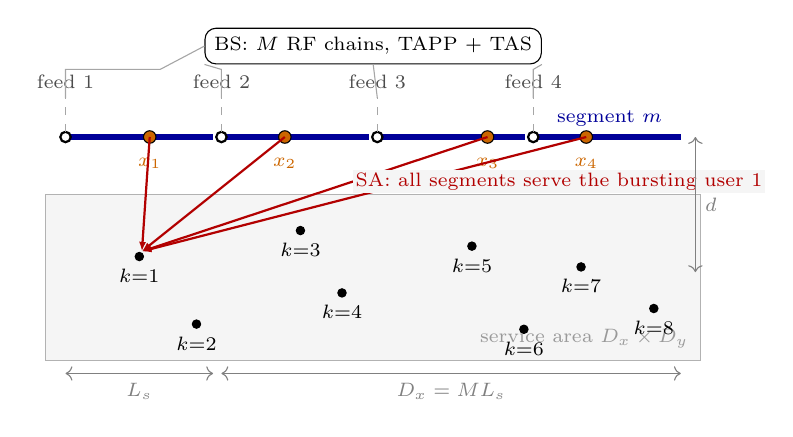
\begin{tikzpicture}[scale=0.66, every node/.style={font=\scriptsize}]
% ground plane (service area)
\fill[gray!8] (-0.3,-1.7) rectangle (12.3,1.5);
\draw[gray!60] (-0.3,-1.7) rectangle (12.3,1.5);
\node[gray!80, anchor=south east] at (12.25,-1.65) {service area $D_x\times D_y$};
% waveguide segments and feeds
\foreach \m in {0,1,2,3} {
  \draw[line width=2.4pt, color=blue!60!black] ({\m*3+0.08},2.6) -- ({\m*3+2.92},2.6);
  \draw[fill=white, thick] ({\m*3+0.08},2.6) circle (0.1);
  \draw[gray!70, dashed] ({\m*3+0.08},2.7) -- ({\m*3+0.08},3.35);
}
\node[gray!60!black, anchor=south] at (0.08,3.35) {feed 1};
\node[gray!60!black, anchor=south] at (3.08,3.35) {feed 2};
\node[gray!60!black, anchor=south] at (6.08,3.35) {feed 3};
\node[gray!60!black, anchor=south] at (9.08,3.35) {feed 4};
\node[draw, rounded corners, fill=white, minimum height=0.45cm] (bs) at (6,4.35) {BS: $M$ RF chains, TAPP + TAS};
\draw[gray!70] (0.08,3.35) -- (0.08,3.9) -- (1.9,3.9) -- (bs.west);
\draw[gray!70] (3.08,3.35) -- (3.08,3.9) -- (bs.south west);
\draw[gray!70] (6.08,3.35) -- (bs.south);
\draw[gray!70] (9.08,3.35) -- (9.08,3.9) -- (bs.south east);
% activated PAs
\foreach \x/\m in {1.7/1, 4.3/2, 8.2/3, 10.1/4} {
  \draw[fill=orange!80!black] (\x,2.6) circle (0.12);
  \node[below=3pt, orange!80!black] at (\x,2.55) {$x_{\m}$};
}
\node[blue!60!black, anchor=west] at (9.35,2.95) {segment $m$};
% users
\foreach \x/\y/\k in {1.5/0.3/1, 2.6/-1.0/2, 4.6/0.8/3, 5.4/-0.4/4, 7.9/0.5/5, 8.9/-1.1/6, 10.0/0.1/7, 11.4/-0.7/8}
{
  \draw[fill=black] (\x,\y) circle (0.08);
  \node[below=1pt] at (\x,\y) {$k{=}\k$};
}
% SA links to user 1
\foreach \x in {1.7,4.3,8.2,10.1} {\draw[-{Latex[length=1.2mm]}, red!70!black, thick] (\x,2.6) -- (1.55,0.4);}
\node[red!70!black, anchor=west, fill=gray!8, inner sep=1pt] at (5.6,1.75) {SA: all segments serve the bursting user $1$};
% geometry annotations
\draw[<->, gray] (12.2,2.6) -- (12.2,0) node[midway, right] {$d$};
\draw[<->, gray] (0.08,-1.95) -- (2.92,-1.95) node[midway, below] {$L_s$};
\draw[<->, gray] (3.08,-1.95) -- (11.92,-1.95) node[midway, below] {$D_x = M L_s$};
\end{tikzpicture}
\caption{Downlink SWAN with $M=4$ segments. Each segment is fed at its left end by its own RF chain and activates one PA at $x_m$; the BS chooses per slot between segment aggregation (SA, shown) and segment multiplexing (SM).}
\label{fig:system}
\end{figure}

\subsection{SWAN Architecture}
We consider the downlink of a SWAN, illustrated in Fig.~\ref{fig:system}. Following \cite{Ouyang2026SWAN}, $M$ dielectric waveguide segments of length $L_s$ are placed end-to-end along the $x$-axis at height $d$ above the ground plane, so that segment $m\in\Mset=\{1,\dots,M\}$ spans $[(m-1)L_s, mL_s]$ and the service area has length $D_x=ML_s$. The feed point of segment $m$ is located at its left end, $\vect{\psi}_m^0=[(m-1)L_s,0,d]^{\mathrm T}$, and is connected to the BS by an individual RF chain and power amplifier with power budget $\Pmax$. Because the segments are not physically connected, the signal captured or radiated by one segment cannot leak into another, and activating a single PA per segment avoids IAR \cite{Ouyang2026SWAN}. The activated PA of segment $m$ is located at $\vect{\psi}_m=[x_m,0,d]^{\mathrm T}$ with
\begin{equation}
x_m\in\mathcal X_m\triangleq[(m-1)L_s+\epsilon_x,\; mL_s-\epsilon_x],
\end{equation}
where $\epsilon_x$ is a small guard distance from the segment ends. We write $\vect{x}=[x_1,\dots,x_M]^{\mathrm T}$.

PA reconfiguration is a physical operation. With pre-installed PAs that are switched on and off, a change of $x_m$ takes microseconds to milliseconds; with sliding PAs it takes milliseconds to seconds \cite{Liu2026PASSTutorial,Wang2026Roaming,Jiang2026DiscreteCoupling}. We model a reconfiguration of segment $m$ as a silence of $\tau_r$ slots of that segment, during which it neither transmits nor receives. Time is slotted with slot duration $T_s$ and index $t=0,1,\dots$; slots are grouped into frames of $T_f\gg\tau_r$ slots. The proposed scheme changes $\vect x$ only at frame boundaries, whereas the reactive benchmark of Section~\ref{sec:results} changes it within frames and pays $\tau_r$ at every change.

\subsection{Users and Channel Model}
$K$ single-antenna HRLLC users, indexed by $k\in\Kset=\{1,\dots,K\}$, are located at $\vect{u}_k=[x_k,y_k,0]^{\mathrm T}$, uniformly distributed in $[0,D_x]\times[-D_y/2,D_y/2]$, and quasi-static within a frame; their positions are known at the BS (e.g., from the localization capability of PASS \cite{Shan2026SWANAccess}). As in the PASS literature \cite{Ding2025FlexibleAntenna,Ouyang2026SWAN}, the link between the PA of segment $m$ and user $k$ is LoS dominated, and the composite channel comprises the free-space path, the in-waveguide propagation from the feed to the PA, and the in-waveguide attenuation:
\begin{equation}\label{eq:channel}
h_{k,m}(x_m)=\frac{\sqrt{\eta}\,e^{-\alpha_g \ell_m}}{r_{k,m}}\exp\!\Big(-\mathrm j\frac{2\pi}{\lambda}\big(r_{k,m}+\neff\,\ell_m\big)\Big),
\end{equation}
where $r_{k,m}=\|\vect u_k-\vect\psi_m\|=\sqrt{(x_k-x_m)^2+y_k^2+d^2}$, $\ell_m=x_m-(m-1)L_s$ is the feed-to-PA distance, $\eta=c^2/(16\pi^2 f_c^2)$ with carrier frequency $f_c$ and speed of light $c$, $\lambda=c/f_c$, $\neff$ is the effective refractive index of the waveguide, and $\alpha_g=\kappa\ln 10/20$ is the amplitude attenuation constant for a waveguide loss of $\kappa$ dB/m. Since $\ell_m\le L_s$, the in-waveguide loss of a SWAN is bounded by $\kappa L_s$ dB irrespective of $D_x$, which is one of the motivations for segmentation \cite{Ouyang2026SWAN}. We collect the channels of user $k$ in $\vect h_k(\vect x)=[h_{k,1}(x_1),\dots,h_{k,M}(x_M)]^{\mathrm T}\in\C^{M}$ and define $\vect H_{\Sset}(\vect x)=[\vect h_k(\vect x)]_{k\in\Sset}^{\mathrm H}\in\C^{|\Sset|\times M}$ for a user subset $\Sset\subseteq\Kset$. To assess robustness to non-LoS scattering, the simulations optionally add a Rician component with $K$-factor $\kappa_R$, $h_{k,m}\leftarrow\sqrt{\tfrac{\kappa_R}{1+\kappa_R}}h_{k,m}+\sqrt{\tfrac{1}{1+\kappa_R}}|h_{k,m}|g_{k,m}$ with $g_{k,m}\sim\mathcal{CN}(0,1)$; the design itself uses \eqref{eq:channel}.

\subsection{Transmission Modes and Finite-Blocklength Coding}
All segments share the same band of $B$ Hz, and a slot carries $n=BT_s$ channel uses. In slot $t$ the BS selects a subset $\Sset[t]\subseteq\Kset$ of at most $M$ users and serves them with linear precoding across the $M$ segment feeds. Two modes arise naturally.

\subsubsection{Segment aggregation (SA)} If $|\Sset|=1$, all segments coherently serve the single user $k$. Under per-segment power constraints the optimal transmission is equal-gain: every segment transmits at power $\rho\Pmax$ with its phase aligned to the user, where $\rho\in(0,1]$ is a power-control factor, and the received SNR is
\begin{equation}\label{eq:snr_sa}
\gamma_k^{\mathrm{SA}}(\vect x,\rho)=\frac{\rho\Pmax}{\sigma^2}\Big(\sum_{m=1}^{M}|h_{k,m}(x_m)|\Big)^2,
\end{equation}
where $\sigma^2$ is the noise power over $B$ Hz.

\subsubsection{Segment multiplexing (SM)} If $2\le|\Sset|\le M$, the BS applies zero-forcing (ZF) precoding $\vect W_{\Sset}=\vect H_{\Sset}^{\mathrm H}(\vect H_{\Sset}\vect H_{\Sset}^{\mathrm H})^{-1}$, whose columns $\vect w_j$ satisfy $\vect h_k^{\mathrm H}\vect w_j=\mathbb 1\{k=j\}$, and allocates the same power $p$ to every stream, so that segment $m$ radiates $p\sum_{j\in\Sset}|w_{m,j}|^2$. The largest $p$ that respects all per-segment budgets is $p(\Sset)=\Pmax/\max_m\sum_{j\in\Sset}|w_{m,j}|^2$, and every user in $\Sset$ enjoys the interference-free SNR
\begin{equation}\label{eq:snr_sm}
\gamma_k^{\mathrm{SM}}(\Sset,\vect x,\rho)=\frac{\rho\,p(\Sset)}{\sigma^2},\qquad k\in\Sset,
\end{equation}
with total radiated power $P_{\mathrm{tot}}(\Sset,\rho)=\rho\,p(\Sset)\sum_{m}\sum_{j\in\Sset}|w_{m,j}|^2$. Equal-SNR ZF is chosen for its closed form; it makes the per-slot decision depend on the subset only through the two scalars $p(\Sset)$ and $P_{\mathrm{tot}}(\Sset,1)$, which are computed once per frame for every subset (Section~\ref{sec:scheme}).

\subsubsection{Finite-blocklength transmission} Packets have $L$ bits. If user $k\in\Sset$ is served with $b_k$ packets in slot $t$, they are jointly encoded into one codeword of $n$ channel uses at rate $R_k=b_kL/n$ bits per channel use. With the normal approximation \cite{Polyanskiy2010}, the decoding error probability at SNR $\gamma$ is
\begin{equation}\label{eq:fbl}
\varepsilon(b,\gamma)=Q\!\left(\Big(\log_2(1+\gamma)-\frac{bL}{n}+\frac{\log_2 n}{2n}\Big)\sqrt{\frac{n}{V(\gamma)}}\right),
\end{equation}
with channel dispersion $V(\gamma)=\big(1-(1+\gamma)^{-2}\big)\log_2^2 e$. A decoding failure is detected through the cyclic redundancy check and reported over an error-free feedback channel; the $b_k$ packets then remain in the queue and are eligible for retransmission in the next slot. Bundling more packets into a codeword raises the rate and hence $\varepsilon$, so the choice of $b_k$ is a reliability--throughput trade-off that is central to HRLLC \cite{Zhao2022QueueAware,Li2024RLR}; TAS resolves it per slot and per user.

\subsection{Bursty Traffic and Deadline-Constrained Queues}
Packets of user $k$ arrive according to a Markov-modulated ON--OFF process, the standard model of bursty sources \cite{Anick1982,Elwalid1993,Ozmen2016}. The source alternates between an ON state, in which packets arrive as a Poisson process with $h_k$ packets per slot (peak rate $h_k/T_s$), and an OFF state without arrivals; the ON$\to$OFF and OFF$\to$ON transition rates are $\alpha_k$ and $\beta_k$ (in s$^{-1}$), so that the mean ON and OFF durations are $1/\alpha_k$ and $1/\beta_k$ and the mean arrival rate is $\bar\lambda_k=h_k\beta_k/(\alpha_k+\beta_k)$ packets per slot. Users may belong to different classes: \emph{critical} users with a larger peak rate and a tighter tail target, and \emph{regular} users. For robustness, Section~\ref{sec:results} also considers Poisson arrivals and the periodic-with-jitter model of industrial control \cite{3GPP-TS22104} superposed with event-triggered bursts.

Each user has a first-in-first-out queue at the BS. Let $A_k[t]$ be the number of arrivals of user $k$ in slot $t$ and $s_k[t]\in\{0,b_k[t]\}$ the number of packets delivered (zero if user $k$ is not scheduled or its codeword is not decoded). The delay $D$ of a packet is the time from its arrival to its successful delivery, measured in slots and counting the transmission slot. HRLLC packets are useless after their budget: a packet whose delay would exceed $\Dmax$ is discarded and counted as a violation, which is the deadline-dropping discipline of \cite{Zhang2025HRL}. Denoting by $q_k[t,a]$ the number of packets of user $k$ with age $a\in\{0,\dots,\Dmax-1\}$ at the beginning of slot $t$, the backlog is $Q_k[t]=\sum_a q_k[t,a]$ and the head-of-line (HoL) age is $\omega_k[t]=\max\{a: q_k[t,a]>0\}$.

\subsection{Tail-Latency Metric}
The HRLLC requirement of user $k$ is the pair $(\Dmax,\delta_k)$: the long-run fraction of packets that are delivered later than $\Dmax$ or discarded must not exceed $\delta_k$,
\begin{equation}\label{eq:tail}
P_k^{\mathrm v}\triangleq\lim_{T\to\infty}\frac{\sum_{t<T}\big(\text{late}_k[t]+\text{dropped}_k[t]\big)}{\sum_{t<T}A_k[t]}=\Pr\{D_k>\Dmax\}\le\delta_k,
\end{equation}
with $\Dmax\in[0.1,1]$ ms and $\delta_k\in[10^{-7},10^{-5}]$ for HRLLC \cite{ITUR-M2160}. Under deadline dropping, late deliveries do not occur, and $P_k^{\mathrm v}$ is the discard fraction; when a longer discard horizon is simulated to display the whole tail, both terms are counted. Note that $P_k^{\mathrm v}$ accounts for queueing, FBL decoding failures, and scheduling jointly, which is the end-to-end reliability that matters for HRLLC \cite{She2018CrossLayer}.

%=====================================================================
\section{Problem Formulation}\label{sec:problem}
%=====================================================================
The BS controls two sets of variables at different rates. On the frame timescale it chooses the PA positions $\vect x[f]\in\mathcal X_1\times\dots\times\mathcal X_M$ of frame $f$. On the slot timescale it chooses the served subset $\Sset[t]$, the packet counts $\vect b[t]=[b_1[t],\dots,b_K[t]]$ with $b_k[t]\le Q_k[t]$ and $b_k[t]=0$ for $k\notin\Sset[t]$, and the power level $\rho[t]$; the precoder follows from $\Sset[t]$ and $\vect x[f]$ through \eqref{eq:snr_sa}--\eqref{eq:snr_sm}. A policy $\pi$ is the collection of these decisions. The design objective is to meet the tail targets of all users while spending as little power as possible:
\begin{subequations}\label{eq:P1}
\begin{align}
\text{(P1)}\quad\min_{\pi}\quad & \bar P(\pi)\triangleq\lim_{T\to\infty}\frac1T\sum_{t<T}\E\big[P_{\mathrm{tot}}(\Sset[t],\rho[t])\big]\label{eq:P1obj}\\
\text{s.t.}\quad & P_k^{\mathrm v}(\pi)\le\delta_k,\quad\forall k\in\Kset,\label{eq:P1tail}\\
& x_m[f]\in\mathcal X_m,\quad\forall m,f,\label{eq:P1x}\\
& |\Sset[t]|\le M,\quad 0\le b_k[t]\le Q_k[t],\quad\rho[t]\in(0,1],\label{eq:P1sched}\\
& \text{delivery and queue dynamics of Section~\ref{sec:model}}.\label{eq:P1dyn}
\end{align}
\end{subequations}
When the targets cannot all be met, the natural relaxation is to minimize the worst violation probability, $\min_\pi\max_k P_k^{\mathrm v}(\pi)/\delta_k$, which is the metric reported in Section~\ref{sec:results}.

Problem (P1) is a constrained Markov decision problem with a continuous geometric decision ($\vect x$), a combinatorial decision per slot ($2^K$ subsets and $\prod_k Q_k$ packet counts), and constraints \eqref{eq:P1tail} on a probability that has no closed form: the delay of a packet depends on the burst structure of all users, on the SNR tables induced by $\vect x$, on the FBL error of every bundle, and on the scheduler itself. Three observations guide the proposed solution. First, the delay tail of a single bursty source served at a constant rate is characterized in closed form by large-buffer asymptotics \cite{Anick1982,Chang1994}, which yields a scalar rate requirement per user that captures $(h_k,\alpha_k,\beta_k,\Dmax,\delta_k)$ jointly (Section~\ref{sec:creq}). Second, for fixed $\vect x$ the dependence of the slot-level problem on the geometry is entirely through the $O(K^M)$ scalars $\{p(\Sset)\}$, which can be tabulated once per frame. Third, the constraint \eqref{eq:P1tail} can be handled online by virtual queues in the drift-plus-penalty framework \cite{Neely2010}, with the objective \eqref{eq:P1obj} as the penalty, which leads to a per-slot problem that is separable over subsets and users.

%=====================================================================
\section{Proposed Tail-Latency-Aware Scheme: TLA-SWAN}\label{sec:scheme}
%=====================================================================
\begin{figure}[t]
\centering
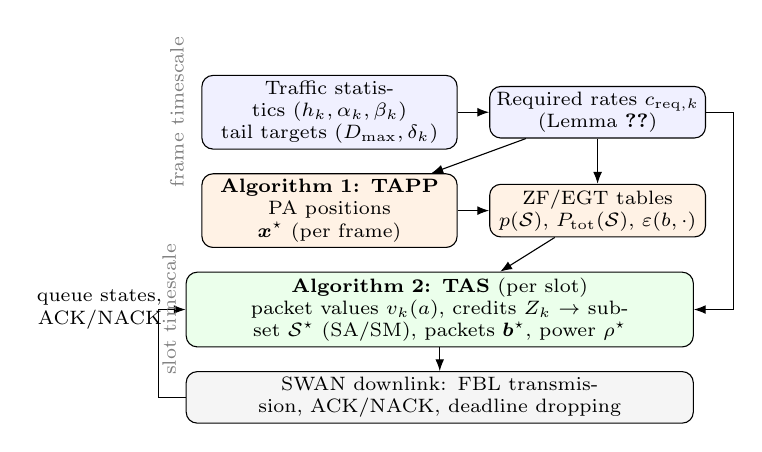
\begin{tikzpicture}[node distance=3mm and 4mm, every node/.style={font=\scriptsize}, box/.style={draw, rounded corners, align=center, minimum height=6mm, inner sep=2pt}]
\node[box, fill=blue!6, text width=3.1cm] (stat) {Traffic statistics $(h_k,\alpha_k,\beta_k)$\\ tail targets $(\Dmax,\delta_k)$};
\node[box, fill=blue!6, text width=2.6cm, right=of stat] (creq) {Required rates $\creqk{k}$\\ (Lemma~\ref{lem:creq})};
\node[box, fill=orange!10, text width=3.1cm, below=of stat] (tapp) {\textbf{Algorithm~1: TAPP}\\ PA positions $\vect x^\star$ (per frame)};
\node[box, fill=orange!10, text width=2.6cm, right=of tapp] (tab) {ZF/EGT tables\\ $p(\Sset)$, $P_{\mathrm{tot}}(\Sset)$, $\varepsilon(b,\cdot)$};
\node[box, fill=green!8, text width=6.3cm, below=of tapp, xshift=1.4cm] (tas) {\textbf{Algorithm~2: TAS} (per slot)\\ packet values $v_k(a)$, credits $Z_k$ $\to$ subset $\Sset^\star$ (SA/SM), packets $\vect b^\star$, power $\rho^\star$};
\node[box, fill=gray!8, text width=6.3cm, below=of tas] (phy) {SWAN downlink: FBL transmission, ACK/NACK, deadline dropping};
\draw[-{Latex[length=1.5mm]}] (stat) -- (creq);
\draw[-{Latex[length=1.5mm]}] (creq) -- (tapp);
\draw[-{Latex[length=1.5mm]}] (creq) -- (tab);
\draw[-{Latex[length=1.5mm]}] (tapp) -- (tab);
\draw[-{Latex[length=1.5mm]}] (tab) -- (tas);
\draw[-{Latex[length=1.5mm]}] (creq.east) -- ++(0.35,0) |- (tas.east);
\draw[-{Latex[length=1.5mm]}] (tas) -- (phy);
\draw[-{Latex[length=1.5mm]}] (phy.west) -- ++(-0.35,0) |- (tas.west) node[pos=0.75, left, align=right] {queue states,\\ ACK/NACK};
\node[left=1mm of stat, rotate=90, anchor=south, gray] {frame timescale};
\node[left=1mm of tas, rotate=90, anchor=south, gray, yshift=-1mm] {slot timescale};
\end{tikzpicture}
\caption{Structure of TLA-SWAN. The tail-latency-aware required rates $\creqk{k}$ couple the frame-level placement and the slot-level scheduler.}
\label{fig:scheme}
\end{figure}

TLA-SWAN, sketched in Fig.~\ref{fig:scheme}, decomposes (P1) along its two timescales. Section~\ref{sec:creq} introduces the required-rate mapping, Section~\ref{sec:tapp} the frame-level placement (Algorithm~\ref{alg:tapp}), Section~\ref{sec:tas} the slot-level scheduler (Algorithm~\ref{alg:tas}), and Section~\ref{sec:complexity} the complexity and signaling. The mathematical statements are given with their proofs deferred to the appendices.

\subsection{Tail-Latency-Aware Required Service Rate}\label{sec:creq}
Consider a single ON--OFF source with parameters $(h,\alpha,\beta)$ served by a constant-rate server of $c$ packets per slot, $\bar\lambda<c<h$. Large-buffer asymptotics of Markov fluid queues \cite{Anick1982,Elwalid1993,Chang1994} state that the stationary workload $W$ satisfies $\Pr\{W>w\}\doteq e^{-\theta^\star(c)\,w}$, where $\theta^\star(c)$ is the unique positive root of $\mathrm{EB}(\theta)=c$ and $\mathrm{EB}(\theta)$ is the effective bandwidth of the source. Since a FIFO packet arriving to workload $W$ experiences delay $W/c$, the delay-violation probability is $\Pr\{D>\Dmax\}\doteq e^{-\theta^\star(c)\,c\,\Dmax}$. Imposing $\Pr\{D>\Dmax\}\le\delta$ and solving for the smallest admissible $c$ gives the following.

\begin{lemma}[Tail-latency-aware required rate]\label{lem:creq}
For an ON--OFF source with peak rate $h$, ON$\to$OFF rate $\alpha$ and OFF$\to$ON rate $\beta$, the effective bandwidth is
$\mathrm{EB}(\theta)=\frac{1}{2\theta}\big[h\theta-\alpha-\beta+\sqrt{(h\theta-\alpha-\beta)^2+4\beta h\theta}\big]$, the decay rate at service rate $c\in(\bar\lambda,h)$ is
\begin{equation}\label{eq:theta}
\theta^\star(c)=\frac{(\alpha+\beta)c-\beta h}{c\,(h-c)},
\end{equation}
and the smallest constant service rate for which the large-buffer approximation of $\Pr\{D>\Dmax\}$ does not exceed $\delta$ is
\begin{equation}\label{eq:creq}
\creq(h,\alpha,\beta,\Dmax,\delta)=h\,\frac{\beta+\Lambda}{\alpha+\beta+\Lambda},\qquad\Lambda\triangleq\frac{\ln(1/\delta)}{\Dmax}.
\end{equation}
\end{lemma}
\todobox{Co-author: prove Lemma~\ref{lem:creq} in Appendix~A (spectral radius of the $2\times2$ generator plus rate matrix, the root of $\mathrm{EB}(\theta)=c$, and the inversion of $\theta^\star(c)\,c=\Lambda$). State precisely in which sense $\doteq$ holds (Chang's large-deviation bound, or the exact Anick--Mitra--Sondhi prefactor for a single source) and add the discrete-time/Poisson-in-ON correction if needed.}

The required rate has the expected limits: $\creq\to\bar\lambda$ when $\Lambda\to0$ (loose target), and $\creq\to h$ when $\Lambda\to\infty$ (stringent target); it increases with $h$, with the burst duration $1/\alpha$, with $\ln(1/\delta)$, and with $1/\Dmax$. Fig.~\ref{fig:creq} illustrates \eqref{eq:creq}. The scalar $\creqk{k}=\creq(h_k,\alpha_k,\beta_k,\Dmax,\delta_k)$ is the only traffic-related quantity used by both algorithms below; it can be updated online from estimates of $(h_k,\alpha_k,\beta_k)$, and Section~\ref{sec:results} shows that TLA-SWAN tolerates a mismatch of a factor of two.

\begin{figure}[t]
\centering
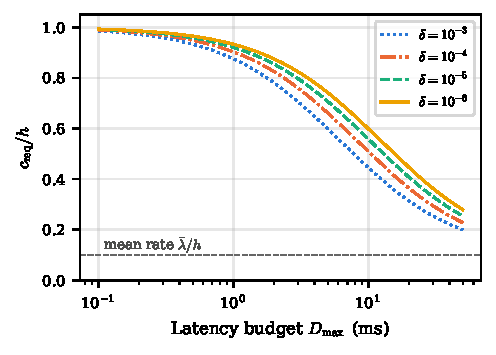
\includegraphics[width=0.9\columnwidth]{fig_creq}
\caption{Tail-latency-aware required rate \eqref{eq:creq} normalized by the peak rate $h$ versus the latency budget $\Dmax$, for a mean burst duration of $1$ ms, an activity factor $\beta/(\alpha+\beta)=0.1$, and several violation targets $\delta$.}
\label{fig:creq}
\end{figure}

\subsection{Frame Timescale: Tail-Aware PA Placement (TAPP)}\label{sec:tapp}
A burst of user $k$ is drained fastest when the SWAN aggregates all segments towards $k$, so the SA rate is the relevant capacity for the delay tail. Let
\begin{equation}\label{eq:Rsa}
R_k^{\mathrm{SA}}(\vect x)=\frac{n}{L}\Big[\log_2\!\big(1+\gamma_k^{\mathrm{SA}}(\vect x,1)\big)-\sqrt{\tfrac{V(\gamma_k^{\mathrm{SA}})}{n}}\,Q^{-1}(\varepsilon_0)+\tfrac{\log_2 n}{2n}\Big]
\end{equation}
be the FBL rate of user $k$ in packets per slot at the nominal reliability $\varepsilon_0$ \cite{Polyanskiy2010}. We define the \emph{tail-latency margin} of user $k$ as $\Gamma_k(\vect x)=R_k^{\mathrm{SA}}(\vect x)/\creqk{k}$: a margin below one means that even exclusive service cannot meet the tail target, while a large margin leaves room for multiplexing with other users. TAPP maximizes the worst margin,
\begin{equation}\label{eq:P2}
\text{(P2)}\quad\max_{\vect x\in\mathcal X_1\times\dots\times\mathcal X_M}\ \min_{k\in\Kset}\ \frac{R_k^{\mathrm{SA}}(\vect x)}{\creqk{k}}.
\end{equation}
Problem (P2) is non-convex and non-smooth, but each coordinate $x_m$ enters $\gamma_k^{\mathrm{SA}}$ only through $|h_{k,m}(x_m)|=\sqrt\eta e^{-\alpha_g\ell_m}/r_{k,m}$, a smooth one-dimensional function on the interval $\mathcal X_m$. This structure suggests block-coordinate descent (BCD) with an exact one-dimensional search per block, as in Algorithm~\ref{alg:tapp}. The one-dimensional problem is solved by a grid of $G$ points followed by local refinement; for a single dominant user per segment it has a closed form.

\begin{algorithm}[t]
\caption{Tail-Aware PA Placement (TAPP), executed once per frame}
\label{alg:tapp}
\begin{algorithmic}[1]
\REQUIRE user positions $\{\vect u_k\}$, required rates $\{\creqk{k}\}$, grid size $G$, tolerance $\xi$
\STATE Initialize $x_m\leftarrow(m-\tfrac12)L_s$ for all $m$; $\Gamma\leftarrow\min_k\Gamma_k(\vect x)$
\REPEAT
  \STATE $\Gamma_{\mathrm{prev}}\leftarrow\Gamma$
  \FOR{$m=1$ \TO $M$}
     \STATE Evaluate $\Gamma^{(g)}=\min_k\Gamma_k(x_1,\dots,x_m^{(g)},\dots,x_M)$ on the grid $\{x_m^{(g)}\}_{g=1}^{G}\subset\mathcal X_m$
     \STATE $g^\star\leftarrow\arg\max_g\Gamma^{(g)}$; \textbf{if} $\Gamma^{(g^\star)}>\Gamma+\xi$ \textbf{then} $x_m\leftarrow x_m^{(g^\star)}$, $\Gamma\leftarrow\Gamma^{(g^\star)}$
  \ENDFOR
\UNTIL{$\Gamma-\Gamma_{\mathrm{prev}}\le\xi$}
\ENSURE $\vect x^\star=\vect x$; if any segment moved, silence it for $\tau_r$ slots
\end{algorithmic}
\end{algorithm}

\begin{lemma}[Closed-form single-user placement]\label{lem:single}
If the margin of user $k$ is the active minimum in (P2) and only $x_m$ is optimized, the optimal position is the projection of the user onto the segment corrected by the in-waveguide attenuation,
$x_m^\star=\Pi_{\mathcal X_m}\big(x_k-\zeta_m\big)$ with $\zeta_m\ge0$ solving a cubic equation, and $x_m^\star=\Pi_{\mathcal X_m}(x_k)$ when $\alpha_g=0$. If two users $k,j$ share the active minimum, $x_m^\star$ equalizes their margins and is the root of a quadratic equation in $x_m$.
\end{lemma}
\todobox{Co-author: derive Lemma~\ref{lem:single} in Appendix~B from $\partial|h_{k,m}|^2/\partial x_m=0$ (with and without $\alpha_g$) and from $\Gamma_k(\vect x)=\Gamma_j(\vect x)$ using the monotonicity of $R^{\mathrm{SA}}$ in $\gamma$; give the explicit coefficients.}

\begin{proposition}[Convergence and complexity of TAPP]\label{prop:tapp}
The sequence of objective values generated by Algorithm~\ref{alg:tapp} is non-decreasing and bounded, hence convergent, and the algorithm terminates after a finite number of sweeps for any $\xi>0$. Each sweep costs $O(MGK)$ evaluations of \eqref{eq:Rsa}, and the output is a coordinate-wise optimal point of (P2) on the grid.
\end{proposition}
\todobox{Co-author: prove Proposition~\ref{prop:tapp} in Appendix~C (monotone bounded sequence; finiteness from $\xi$ and the boundedness of the objective by $\max_k R_k^{\mathrm{SA}}/\creqk{k}$ evaluated at $r_{k,m}=d$); discuss whether a limit point in the continuous domain is a stationary point of the max-min objective.}

\begin{remark}
TAPP differs from rate-maximizing placement in two ways. It is max-min rather than sum, so no user is sacrificed, and the margins are normalized by $\creqk{k}$, so a critical or bursty user attracts PAs even if its channel is already good. In the homogeneous case ($\creqk{k}=\creq$ for all $k$) TAPP reduces to max-min SA-rate placement; the difference becomes visible with heterogeneous classes (Section~\ref{sec:results}).
\end{remark}

\subsection{Slot Timescale: Tail-Aware Scheduling (TAS)}\label{sec:tas}
\subsubsection{Virtual credits}
Constraint \eqref{eq:P1tail} is a long-term constraint on a tail probability and cannot be enforced by a per-slot rule directly. Following the persistent-service-queue construction of \cite{Neely2013DelayNUM}, we replace it by the requirement that user $k$ receive service at rate $\creqk{k}$ whenever it is backlogged, and we track the deficit with a virtual credit $Z_k[t]$,
\begin{equation}\label{eq:Z}
Z_k[t+1]=\min\Big\{\big[Z_k[t]+\creqk{k}\mathbb 1\{Q_k[t]>0\}-s_k[t]\big]^+,\;Z_k^{\max}\Big\},
\end{equation}
with cap $Z_k^{\max}=\creqk{k}\Dmax$, the credit needed to drain one deadline window. $Z_k$ grows while a backlogged user is served below its required rate, is repaid when it is served above it, and does not change while the user is idle; it measures, in packets, how far the current backlog period is behind the tail-aware drain schedule. In units of time, $Z_k/\creqk{k}$ is the number of slots by which the user is late.

\subsubsection{Packet values}
The Lyapunov drift of $\tfrac12\sum_k Z_k^2$ yields a weight proportional to $Z_k$ on the service $s_k$, i.e., a max-weight rule with the credit as weight. A credit-weighted rule, however, is indifferent to \emph{which} packets of a user are served, whereas under deadline dropping the packets closest to expiry are the ones that will be lost. We therefore combine the credit with an age-dependent packet value in the spirit of the exponential and largest-weighted-delay-first rules \cite{Shakkottai2002EXP,Stolyar2001LWDF,Andrews2001}: a packet of user $k$ with age $a$ (delay $a+1$ if delivered now) carries the value
\begin{equation}\label{eq:value}
v_k(a)=\exp\!\Big(a_k\Big[a+1+\zeta\frac{Z_k[t]}{\creqk{k}}-\Dmax\Big]\Big),\qquad a_k=\frac{\ln(1/\delta_k)}{\Dmax},
\end{equation}
where $\zeta\ge0$ weighs the credit. The exponent $a_k$ is the M-LWDF/LWDF weight that makes the rule large-deviations optimal for the delay-tail exponents of all users \cite{Stolyar2001LWDF,Andrews2001}: a packet at its deadline has value one, a fresh packet has value $\delta_k$, and a user that is $Z_k/\creqk{k}$ slots behind schedule sees all its packets aged by that amount. Serving the $b$ oldest packets of user $k$ yields the value $U_k(b)=\sum_{i=1}^{b}v_k(a_{k,(i)})$, where $a_{k,(1)}\ge a_{k,(2)}\ge\dots$ are the ages in FIFO order.

\subsubsection{Per-slot problem}
Since a codeword either delivers all its packets or none, the expected value collected from user $k$ in subset $\Sset$ at power level $\rho$ is $(1-\varepsilon(b_k,\gamma_k(\Sset,\rho)))U_k(b_k)$, where $\gamma_k$ is \eqref{eq:snr_sa} if $|\Sset|=1$ and \eqref{eq:snr_sm} otherwise. Adding the power penalty of the drift-plus-penalty method with parameter $V\ge0$, the slot-level problem is
\begin{equation}\label{eq:P3}
\text{(P3)}\ \max_{\Sset,\vect b,\rho}\ \sum_{k\in\Sset}\big(1-\varepsilon(b_k,\gamma_k(\Sset,\rho))\big)U_k(b_k)-V\,P_{\mathrm{tot}}(\Sset,\rho),
\end{equation}
subject to \eqref{eq:P1sched}. For fixed $(\Sset,\rho)$, (P3) separates over users, and the optimal bundle size of user $k$ is
\begin{equation}\label{eq:bstar}
b_k^\star(\Sset,\rho)=\arg\max_{1\le b\le\min\{Q_k,b_{\max}\}}\big(1-\varepsilon(b,\gamma_k(\Sset,\rho))\big)U_k(b),
\end{equation}
a one-dimensional integer search with at most $b_{\max}$ candidates, where $b_{\max}$ is the largest number of packets that fits in a slot at the maximum SNR. Because $U_k(b)$ is concave in $b$ and increasing, while $1-\varepsilon$ decreases in $b$, \eqref{eq:bstar} automatically bundles many packets when they are young and sends only the urgent ones, at a lower and more reliable rate, when the oldest packets approach their deadline; this is the tail-aware counterpart of queue-aware FBL coding \cite{Zhao2022QueueAware}. The outer maximization over $(\Sset,\rho)$ is exhaustive: $\gamma_k(\Sset,\rho)$ depends on $(\Sset,\rho)$ only through $\rho p(\Sset)$, and the error terms $\varepsilon(b,\rho p(\Sset)/\sigma^2)$ for all $b\le b_{\max}$, all subsets, and all $\rho$ in a finite set $\mathcal R$ are tabulated once per frame. With the tables in memory, evaluating (P3) for all $\sum_{s\le M}\binom{K}{s}$ subsets is a vectorized lookup, which is feasible for $K\le 12$ and $M\le 8$ within a fraction of a slot; for larger $K$ a greedy subset construction can be used with a loss that is reported in Section~\ref{sec:results}. The choice $|\Sset^\star|=1$ corresponds to SA and $|\Sset^\star|\ge2$ to SM, so the mode selection is a by-product of (P3) rather than a separate rule: the scheduler aggregates the segments when one user is far behind its tail schedule, and multiplexes when several users hold packets of comparable urgency.

\begin{algorithm}[t]
\caption{Tail-Aware Scheduling (TAS), executed every slot $t$}
\label{alg:tas}
\begin{algorithmic}[1]
\REQUIRE tables $\{p(\Sset),P_{\mathrm{tot}}(\Sset)\}_{\Sset}$, $\{\varepsilon(b,\rho p(\Sset)/\sigma^2)\}_{b\le b_{\max},\rho\in\mathcal R}$ (from $\vect x^\star$), credits $\{Z_k[t]\}$, age profiles $\{q_k[t,\cdot]\}$, parameters $V,\zeta$
\STATE Admit new arrivals with age $0$; discard packets with age $\ge\Dmax$ and count them as violations
\STATE Compute $v_k(a)$ by \eqref{eq:value} and $U_k(b)$ for $b\le\min\{Q_k,b_{\max}\}$, $\forall k$ with $Q_k>0$
\FOR{every subset $\Sset$ of backlogged users with $|\Sset|\le M$ and every $\rho\in\mathcal R$}
   \STATE $b_k^\star(\Sset,\rho)$ by \eqref{eq:bstar} for $k\in\Sset$; $J(\Sset,\rho)$ by \eqref{eq:P3}
\ENDFOR
\STATE $(\Sset^\star,\rho^\star)\leftarrow\arg\max J(\Sset,\rho)$; transmit $b_k^\star$ packets to each $k\in\Sset^\star$ with EGT if $|\Sset^\star|=1$ and ZF otherwise
\STATE On ACK, remove the $b_k^\star$ oldest packets of $k$ and set $s_k[t]=b_k^\star$; on NACK keep them and set $s_k[t]=0$
\STATE Update the credits by \eqref{eq:Z}; age all remaining packets by one slot
\end{algorithmic}
\end{algorithm}

\subsubsection{Guarantees}
The following statements formalize the behavior of Algorithm~\ref{alg:tas}.
\begin{theorem}[Drift-plus-penalty bound]\label{thm:dpp}
Let the arrivals and the FBL success indicators be such that $A_k[t]\le A_{\max}$ and $s_k[t]\le b_{\max}$, and suppose the required rates are feasible, i.e., there exists a randomized stationary policy that serves every backlogged user at rate at least $\creqk{k}+\epsilon$ for some $\epsilon>0$. Then, under Algorithm~\ref{alg:tas} with $\zeta=0$ and the credit \eqref{eq:Z} without cap, the credits are deterministically bounded, $Z_k[t]\le Z_k^{\mathrm{ub}}(V)$ for all $t$, the time-average power satisfies $\bar P\le\bar P^{\mathrm{opt}}+\mathcal B/V$ for a constant $\mathcal B$, and every packet of user $k$ that is not discarded is delivered within $\lceil(Q_k^{\max}+Z_k^{\mathrm{ub}}(V))/\creqk{k}\rceil$ slots.
\end{theorem}
\todobox{Co-author: prove Theorem~\ref{thm:dpp} in Appendix~D following the persistent-queue argument of \cite[Sec.~IV]{Neely2013DelayNUM} and the drift-plus-penalty bound of \cite[Ch.~4]{Neely2010}; identify $\mathcal B=\tfrac12\sum_k(\creqk{k}^2+b_{\max}^2)$ or tighter; specify $Z_k^{\mathrm{ub}}(V)$ and $Q_k^{\max}$ under deadline dropping ($Q_k^{\max}\le A_{\max}\Dmax$). Extend the statement to $\zeta>0$, or explain why the age-dependent values do not affect the bound (the value $v_k(a)\ge\delta_k$ is bounded away from zero and the objective is a weighted sum of the same service variables).}

\begin{theorem}[Tail bound]\label{thm:tail}
Let $\mu_k(\theta)$ denote the effective capacity \cite{Wu2003,Gursoy2013} of the service process $\{s_k[t]\}$ of user $k$ induced by TLA-SWAN, and let $\mathrm{EB}_k(\theta)$ be the effective bandwidth of its ON--OFF source. If $\theta_k^\star>0$ solves $\mathrm{EB}_k(\theta)=\mu_k(\theta)$, then $\Pr\{D_k>\Dmax\}\le\varsigma_k\,e^{-\theta_k^\star\mathrm{EB}_k(\theta_k^\star)\Dmax}$ with $\varsigma_k=\Pr\{Q_k>0\}\le1$. In particular, if the fraction of slots in which user $k$ is served in SA mode is at least $\phi_k$ and the SA bundle is decoded with probability at least $1-\varepsilon_0$, then $\mu_k(\theta)\ge-\tfrac1\theta\ln\big(1-\phi_k+\phi_k(\varepsilon_0+(1-\varepsilon_0)e^{-\theta b_k^{\mathrm{SA}}})\big)$, where $b_k^{\mathrm{SA}}=\lfloor R_k^{\mathrm{SA}}(\vect x^\star)\rfloor$, which makes the bound computable from the output of Algorithm~\ref{alg:tapp}.
\end{theorem}
\todobox{Co-author: prove Theorem~\ref{thm:tail} in Appendix~E via the effective bandwidth/effective capacity duality \cite{Chang1994,Wu2003} with the FBL service model of \cite{Gursoy2013,Schiessl2018} (i.i.d. success indicators conditioned on the schedule), and justify the lower bound on $\mu_k(\theta)$ by the monotonicity of the effective capacity in the service distribution. Discuss the choice of $\phi_k$ (e.g., $\phi_k=\min\{1,\creqk{k}/b_k^{\mathrm{SA}}\}$ under Theorem~\ref{thm:dpp}) and compare the bound with the simulated tail in Fig.~\ref{fig:ccdf} (to be added once derived).}

\subsection{Complexity and Signaling}\label{sec:complexity}
TAPP runs once per frame with $O(I\,MGK)$ operations, where $I$ is the number of sweeps ($I\le5$ in all our experiments). The per-frame tables require one ZF inversion of size $|\Sset|\times|\Sset|$ per subset, i.e., $O\big(\sum_{s\le M}\binom{K}{s}s^3\big)$, and the FBL error table has $|\mathcal R|\,b_{\max}$ entries per subset; for $K=8$, $M=4$, $|\mathcal R|=5$, $b_{\max}=12$ this is $162$ subsets and about $10^4$ scalars. Per slot, TAS evaluates $U_k(b)$ in $O(K\Dmax)$ and (P3) in $O\big(|\mathcal R|\,b_{\max}\sum_{s\le M}\binom{K}{s}\big)$ vectorized operations, which is a lookup of the order of $10^4$ scalars, i.e., microseconds on a modern processor. Signaling is that of any multi-user MIMO downlink (CSI at the BS, ACK/NACK feedback) plus the traffic statistics of each user, which are three scalars updated on the frame timescale; the PA positions are set by the BS itself.

%=====================================================================
\section{Simulation Results}\label{sec:results}
%=====================================================================
\subsection{Setup and Benchmarks}
We simulate the system of Section~\ref{sec:model} at the slot level, including the FBL decoding errors drawn from \eqref{eq:fbl}, retransmissions, deadline dropping, the reconfiguration silence, and the exact packet ages, with the parameters of Table~\ref{tab:params} unless stated otherwise. The PHY parameters follow the SWAN literature \cite{Ouyang2026SWAN,Gu2026HSSA}; the slot of $0.1$ ms with $n=200$ channel uses corresponds to a $2$-MHz HRLLC carrier and the $32$-byte packets to the 3GPP reference payload \cite{3GPP-TS22261,3GPP-TS22104}. The default traffic is an ON--OFF source with mean burst duration $1/\alpha=1$ ms, activity factor $\beta/(\alpha+\beta)=0.1$, and peak rate $h=3$ packets per slot, i.e., a peak of $7.7$ Mb/s and a mean load of $0.3$ packets per slot per user; for $K=8$ users the mean offered load is $2.4$ packets per slot, whereas a single stream carries between $3$ and $5$ packets per slot depending on the SNR, so that a single burst is drainable but simultaneous bursts overload the system. Each point pools four independent user drops of $2.5\times10^5$ slots ($25$ s) each, i.e., about $2.4\times10^6$ packets per point, so that violation probabilities down to $10^{-5}$ are resolved; the delay tail of Fig.~\ref{fig:ccdf} uses $3.2\times10^6$ slots. Points with zero observed violations are drawn at $1/(\text{number of packets})$.

\begin{table}[t]
\caption{Default simulation parameters}
\label{tab:params}
\centering
\footnotesize
\begin{tabular}{ll|ll}
\toprule
Parameter & Value & Parameter & Value\\
\midrule
Carrier $f_c$ & $28$ GHz & Segments $M$, length $L_s$ & $4$, $10$ m\\
$\neff$, $\kappa$ & $1.4$, $0.08$ dB/m & Height $d$, width $D_y$ & $3$ m, $10$ m\\
Noise $\sigma^2$ ($B=2$ MHz) & $-101$ dBm & Users $K$ & $8$\\
Per-segment power $\Pmax$ & $-10$ dBm & Slot $T_s$, blocklength $n$ & $0.1$ ms, $200$\\
Packet $L$ & $256$ bits & $b_{\max}$, $\mathcal R$ & $12$, $\{1\}$ ($\{0.1,\dots,1\}$ for $V>0$)\\
Peak rate $h$ & $3$ pkt/slot & ON/OFF means $1/\alpha$, $1/\beta$ & $1$ ms, $9$ ms\\
Budget $\Dmax$ & $1$ ms ($10$ slots) & Target $\delta$ & $10^{-5}$\\
Critical users & $h=4$, $\delta=10^{-6}$ & Nominal $\varepsilon_0$ (TAPP) & $10^{-5}$\\
Reconfiguration $\tau_r$ & $1$ slot & TAS $\zeta$, $V$ & see text\\
\bottomrule
\end{tabular}
\end{table}

The following schemes are compared.
\begin{itemize}[leftmargin=*]
\item \textbf{TLA-SWAN}: TAPP placement and TAS scheduling (proposed).
\item \textbf{SWAN, M-LWDF}: TAPP placement with the M-LWDF rule \cite{Andrews2001}, i.e., user weights $a_k\omega_k[t]/\bar r_k[t]$ with $\bar r_k$ the exponentially averaged delivered rate, applied to the same subset search and goodput-maximizing bundling.
\item \textbf{SWAN, max-weight}: TAPP placement with queue-length weights (throughput-optimal, tail-agnostic).
\item \textbf{SWAN, EDF}: TAPP placement with earliest-deadline-first user selection, i.e., the $M$ users with the oldest HoL packets, without channel awareness.
\item \textbf{SWAN, sum-rate + MW}: PA placement maximizing $\sum_k R_k^{\mathrm{SA}}$ (the rate-centric SWAN design \cite{Ouyang2026SWAN,Gu2026SWANSumRate}) with max-weight scheduling.
\item \textbf{SWAN, fixed PAs}: PAs at the segment centers (no reconfiguration) with TAS.
\item \textbf{SWAN, reactive}: every slot, each segment moves its PA above the backlogged user with the largest weight in its range and pays $\tau_r$ slots of silence per move; TAS scheduling.
\item \textbf{Single-waveguide PASS}: one waveguide of length $D_x$ fed at $x=0$ with one RF chain, $M$ PAs at the TAPP positions, in-waveguide loss over the full length, and SA/TDMA only (one user per slot) \cite{Ding2025FlexibleAntenna}.
\item \textbf{Fixed antenna array}: $M$ co-located antennas at $\lambda/2$ spacing at the center of the area at height $d$, ZF precoding, TAS.
\end{itemize}
